%%%%%%%%%%%%%%%%%%%% Preamble %%%%%%%%%%%%%%%%%%%%
\documentclass[10pt, paper=a4]{article}
\usepackage{amssymb,amsfonts,amsmath,latexsym,amsthm, mathtools} %mathtext,
\usepackage{booktabs}
\usepackage{multirow}
\usepackage{graphicx}
\usepackage{listings}
\usepackage{chngpage}
\usepackage[font=footnotesize, labelsep=period]{caption}
\usepackage{cite}
\usepackage[scale=0.925]{geometry}
\graphicspath{{images/}}
\usepackage[pdftex,unicode,colorlinks, citecolor=blue,
  filecolor=black, linkcolor=blue, urlcolor=blue]{hyperref}
\usepackage[figure,table]{hypcap}
%%%%%%%%%%%%%%%%%%%% Document %%%%%%%%%%%%%%%%%%%%
\begin{document}
%%%%%%%%%%%%%%%%%%%% Title page %%%%%%%%%%%%%%%%%%%%
\title{Report 02}

\author{Dmitriy Markovich, Julian Lemos Vinasco}

\date{}

\maketitle

\begin{abstract}
  Objective: The objective of this second report is to apply the
  methods you have learned in the second section of the course on
  ”Supervised learning: Classification and regression” in order to
  solve both a relevant classification and regression problem for your
  data.
\end{abstract}

%%%%%%%%%%%%%%%%%%%% Introduction %%%%%%%%%%%%%%%%%%%%
\section{Regression}
\label{sec:regression}
In this section of the report you are to solve a relevant regression
problem for your data. In particular, you should:
\begin{enumerate}
\item Explain which regression problem you have chosen to solve.
\item Apply linear regression with forward selection and consider if
  transforming or combining attributes potentially may be useful. For
  linear regression, plotting the residual error vs. the attributes
  can give some insight into whether in- cluding a transformation of a
  variable can improve the model, i.e. potentially describe parts of
  the residuals.
\item Explain how a new data observation is predicted according to the
  estimated model. I.e. what are the effects of the selected
  attributes in terms of predicting the data.  (Notice, if you
  interpret the magnitude of the estimated coefficients this in
  general requires that each attribute be normalized prior to the
  analysis).
\item Fit an artificial neural network (ANN) model to the data.
\item Statistically evaluate if there is a significant performance
  difference between the fitted ANN and linear regression models based
  on the same cross-validation splits (i.e., use a paired
  t-test). Compare in addition if the performance of your models are
  better than simply predicting the output to be the average of the
  training data output.
\end{enumerate}

%% Test images from Dmitriy are depicted on Fig.~\ref{fig:test}.
%% \begin{figure}
%%   \begin{minipage}{0.49\textwidth}
%%     
\includegraphics[width = 0.99\textwidth]{download.jpg}
%%   \end{minipage} \hfill
%%   \begin{minipage}{0.49\textwidth}
%%     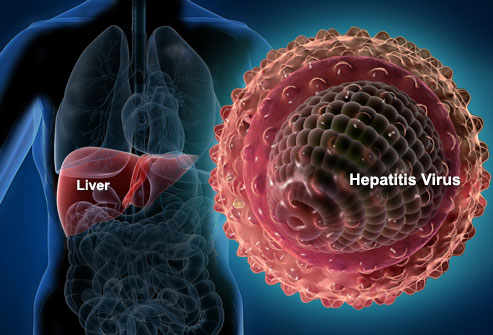
\includegraphics[width = 0.99\textwidth]{webmd_rf_photo_of_liver_and_hepatitis_virus.jpg}
%%   \end{minipage} \vfill
%%   \caption{Test figures of Hepatitis from Dmitriy.}
%%   \label{fig:test}
%% \end{figure}
%%%%%%%%%%%%%%%%%%%% Classification %%%%%%%%%%%%%%%%%%%%
\section{Classification}
\label{sec:classification}

\begin{enumerate}
\item Explain which classification problem you have chosen to solve.
\item Apply at least three of the following methods: Decision Trees
  (as in Fig.~\ref{fig:decision_tree}), Logistic/Multinomial
  Regression (as in Lst.~\ref{lst:logistic_regression}), K-Nearest
  Neighbors (KNN), Naı̈ve Bayes and Artificial Neural Networks (ANN).
  (Use cross-validation to select relevant parameters in an inner
  cross-validation loop and give in a table the performance results
  for the methods evaluated on the same cross-validation splits on the
  outer cross-validation loop, i.e. you should use two levels of
  cross-validation).
\item For the models you are able to interpret explain how a new data
  observation is classified.  (If you have multiple models fitted,
  (i.e., one for each cross-validation split) either focus on one of
  these fitted models or consider fitting one model for the optimal
  setting of the parameters estimated by cross-validation to all the
  data.)
\item Statistically compare the performance of the two best performing
  models (i.e., use a paired t-test). Compare in addition if the
  performance of your models are better than simply predicting all
  outputs to be the largest class in the training data.
\end{enumerate}


The classification problem for the dataset is to predict the age range
of abalones using their measured physical characteristics.  Age in
years as an attribute can be calculated from the Rings attribute as
Age = 1.5 + Rings.  Age range may be obtained from the Age attributes
by splitting it into a number of groups.  Grouping can be done in a
variety of ways, but it is statistically wise to group the data in a
way that the number of counts in each group is at least on the same
scale with the others.  The distribution of Age attribute and its
splitting into 5 groups is presented in Fig.~\ref{fig:age_grouping}.

\begin{figure}[htbp]
  \centering
  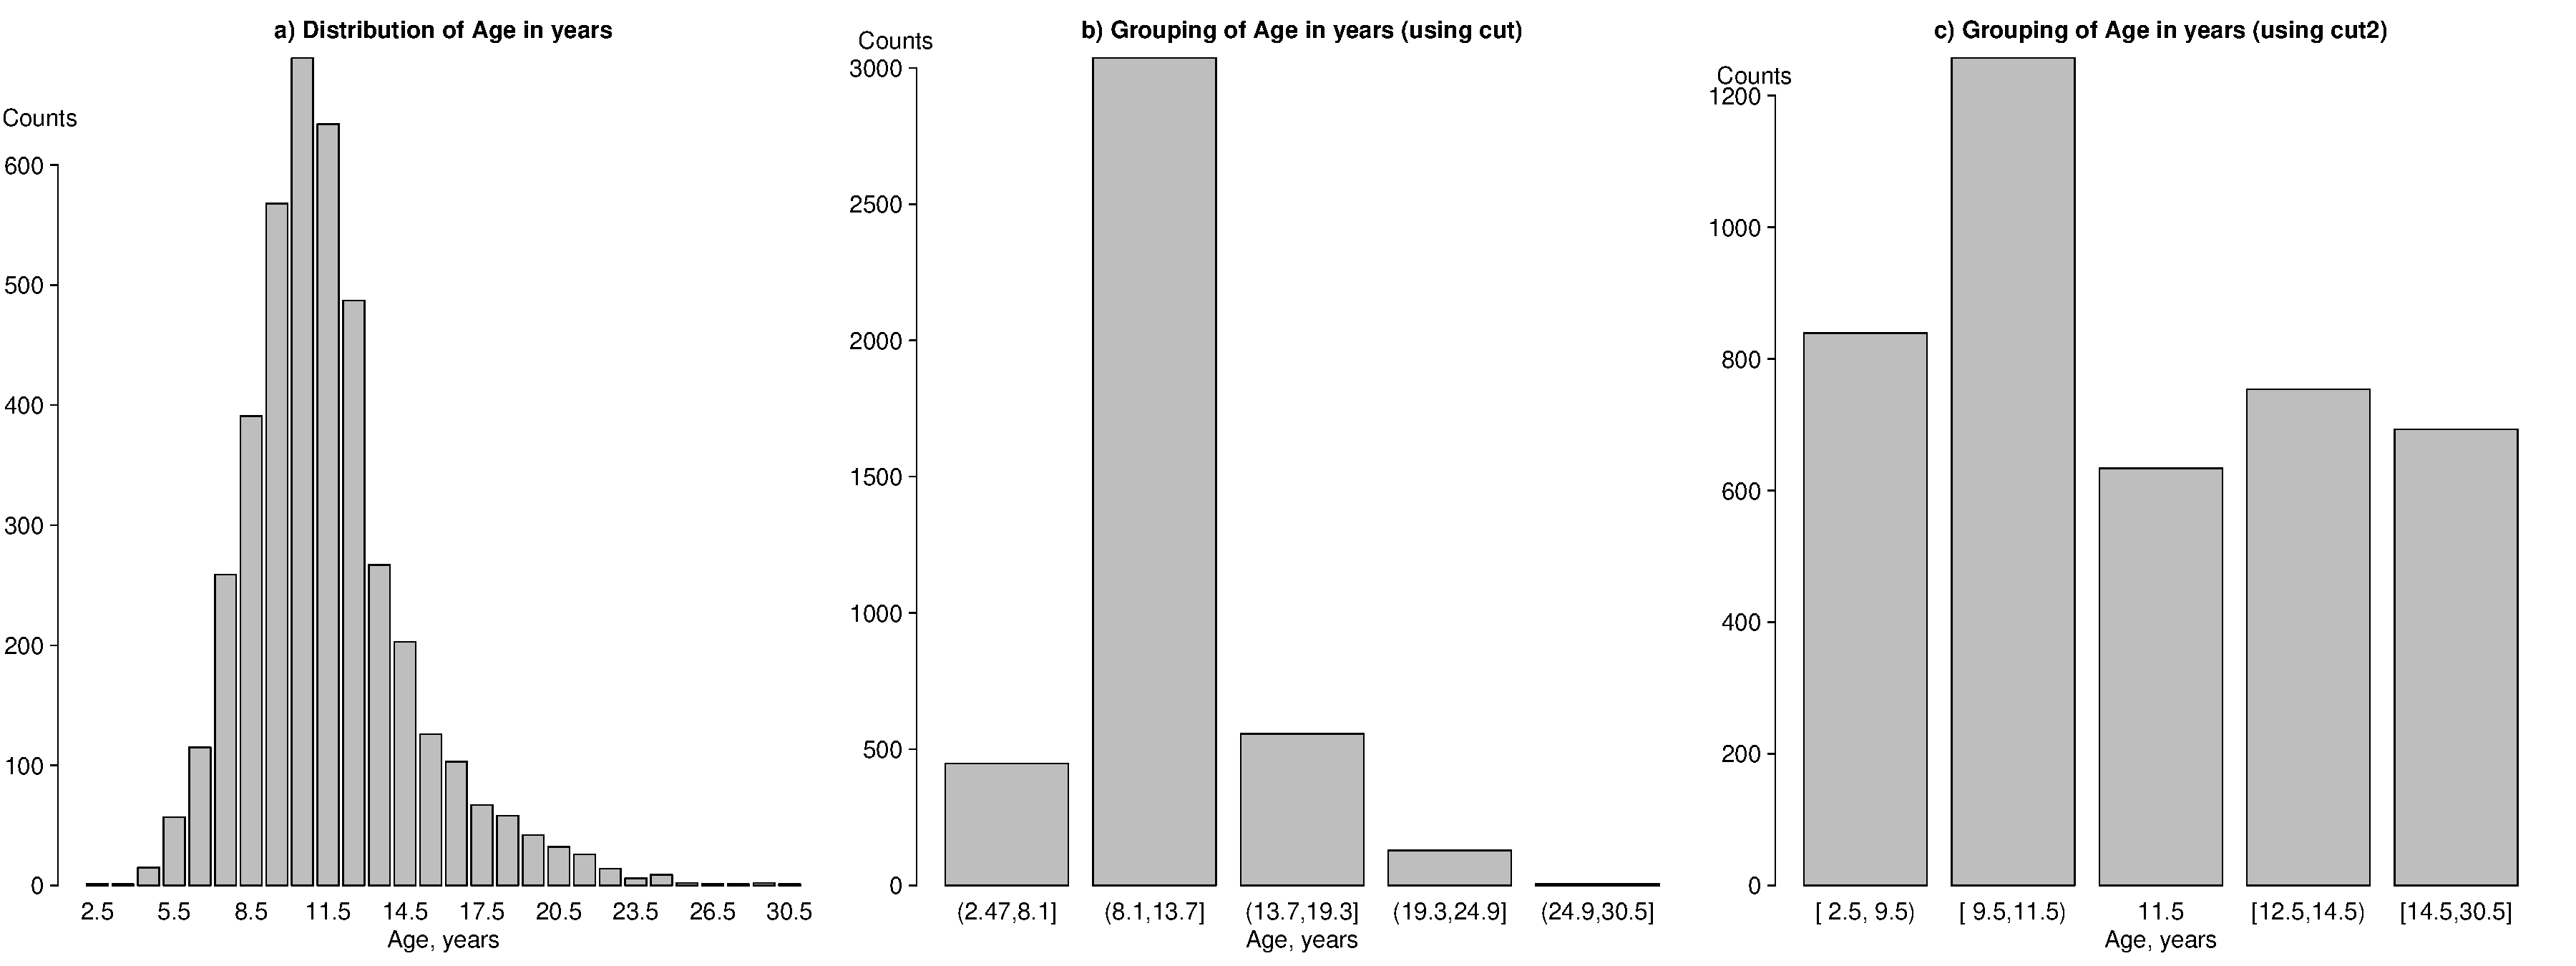
\includegraphics[width = 0.99\textwidth]{age_grouping.pdf}
  \caption{Distribution and grouping of Age attribute.}
  \label{fig:age_grouping}
\end{figure}

Each of the groups in Fig.~\ref{fig:age_grouping} represents a certain
class, that the continuous Age attribute belongs to.  So we can
proceed with predicting the age range or the class of Age using other
attributes with the help of various classification methods.

\subsection{Decision trees}
Decision tree is a tool that uses a tree-like model of decisions and
their possible consequences.  The goal is to find out how on the basis
of all other attributes to classify the age according to splitting in
Fig.~\ref{fig:age_grouping}.  To visualize the idea, the result of
fitting a decision tree to the whole dataset is presented in
Fig.~\ref{fig:decision_tree}.  Pruning level was set to 0.01, minimum
number of observations in the node to attempt splitting --- to 5.
Basically, the tree shows that only two attributes are required to
classify the Age --- ShllWght and ShckdWght.

\begin{figure}[htbp]
  \centering
  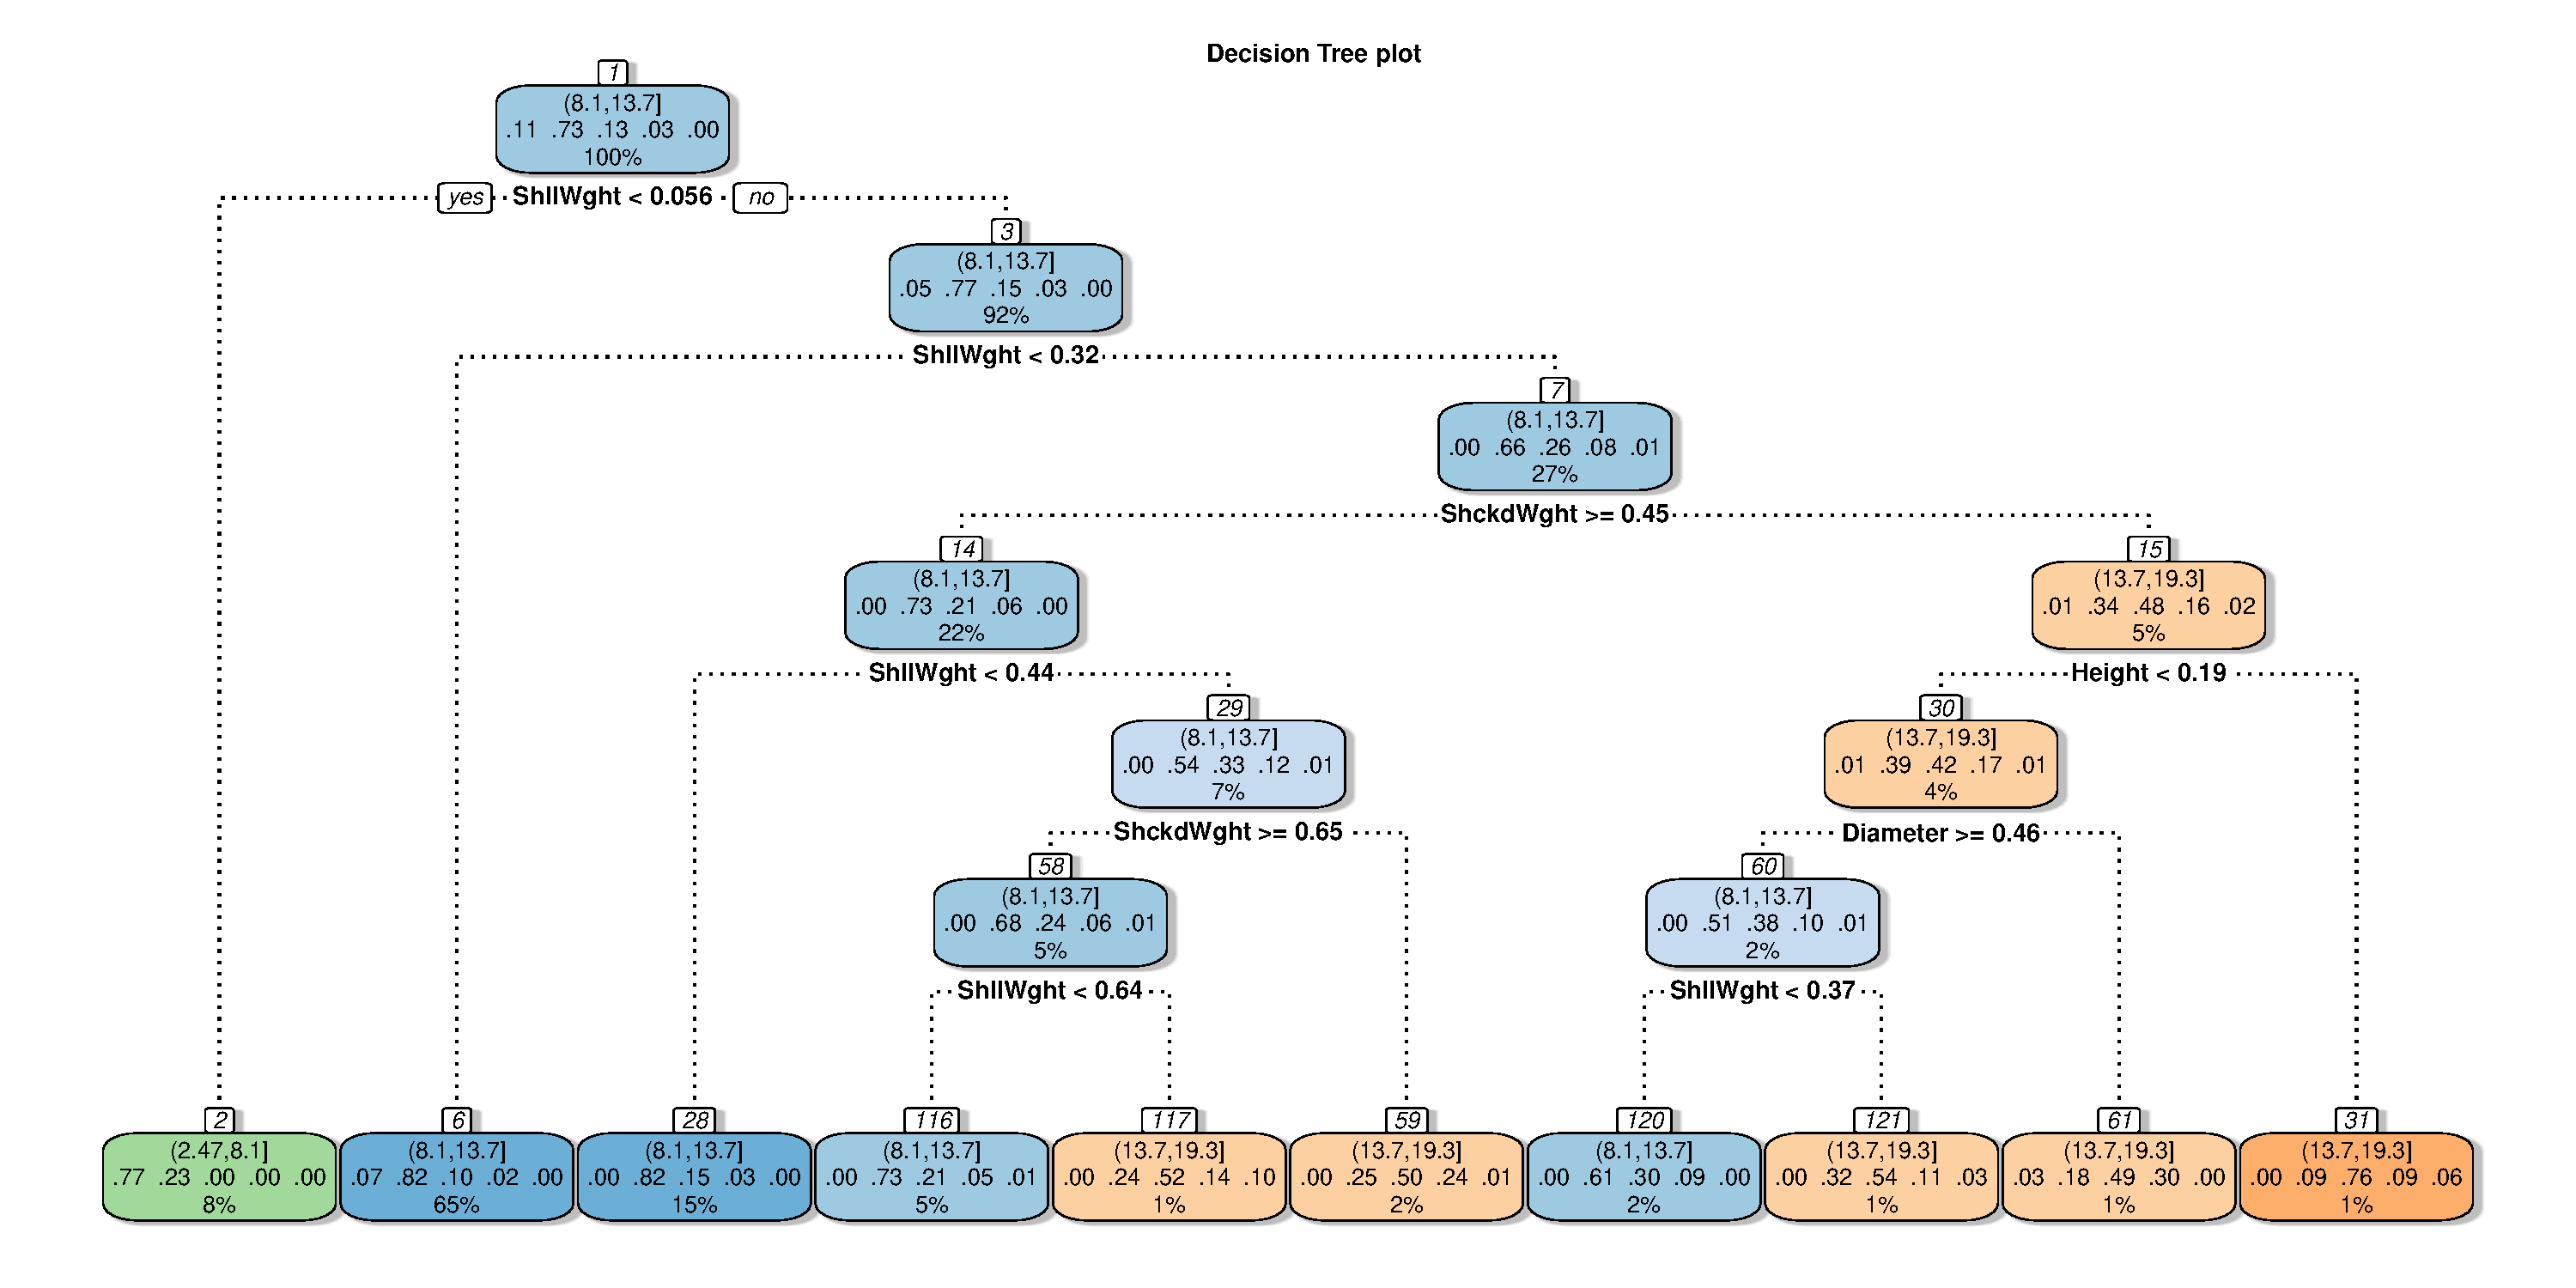
\includegraphics[width = 0.49\textwidth]{decision_tree.pdf}
  \caption{Decision tree fitted to the whole dataset.  Pruning level
    was set to 0.01, minimum number of observations in the node to
    attempt splitting --- to 5.}
  \label{fig:decision_tree}
\end{figure}

The tree in Fig.~\ref{fig:decision_tree} was fitted to the whole
dataset, and there is no way to validate the model.  In practice,
model selecion and performance evaluation of a decision tree are
achieved by two layer cross-validation, where at the outer level the
performance of the optimal model is evaluated and on the inner level
the optimal model is selected.

The complexity of the decision tree model is defined by its pruning
level.  Generally, a full decision tree with pruning level zero turns
to overfitting --- it has a very low error rate on the training
dataset, but a very large error on the test dataset.  Adjusting the
pruning level with one layer K-fold cross-validation gives the optimal
pruning level.  The result of applying one layer 10-fold
cross-validation to the data is presented in Fig.~\ref{fig:cv_1}.
Minimum number of observations in the node to attempt splitting was
set to 5.  The optimal pruning level is 0.0026 and the error rate is
47.7 \%.

\begin{figure}[htbp]
  \centering
  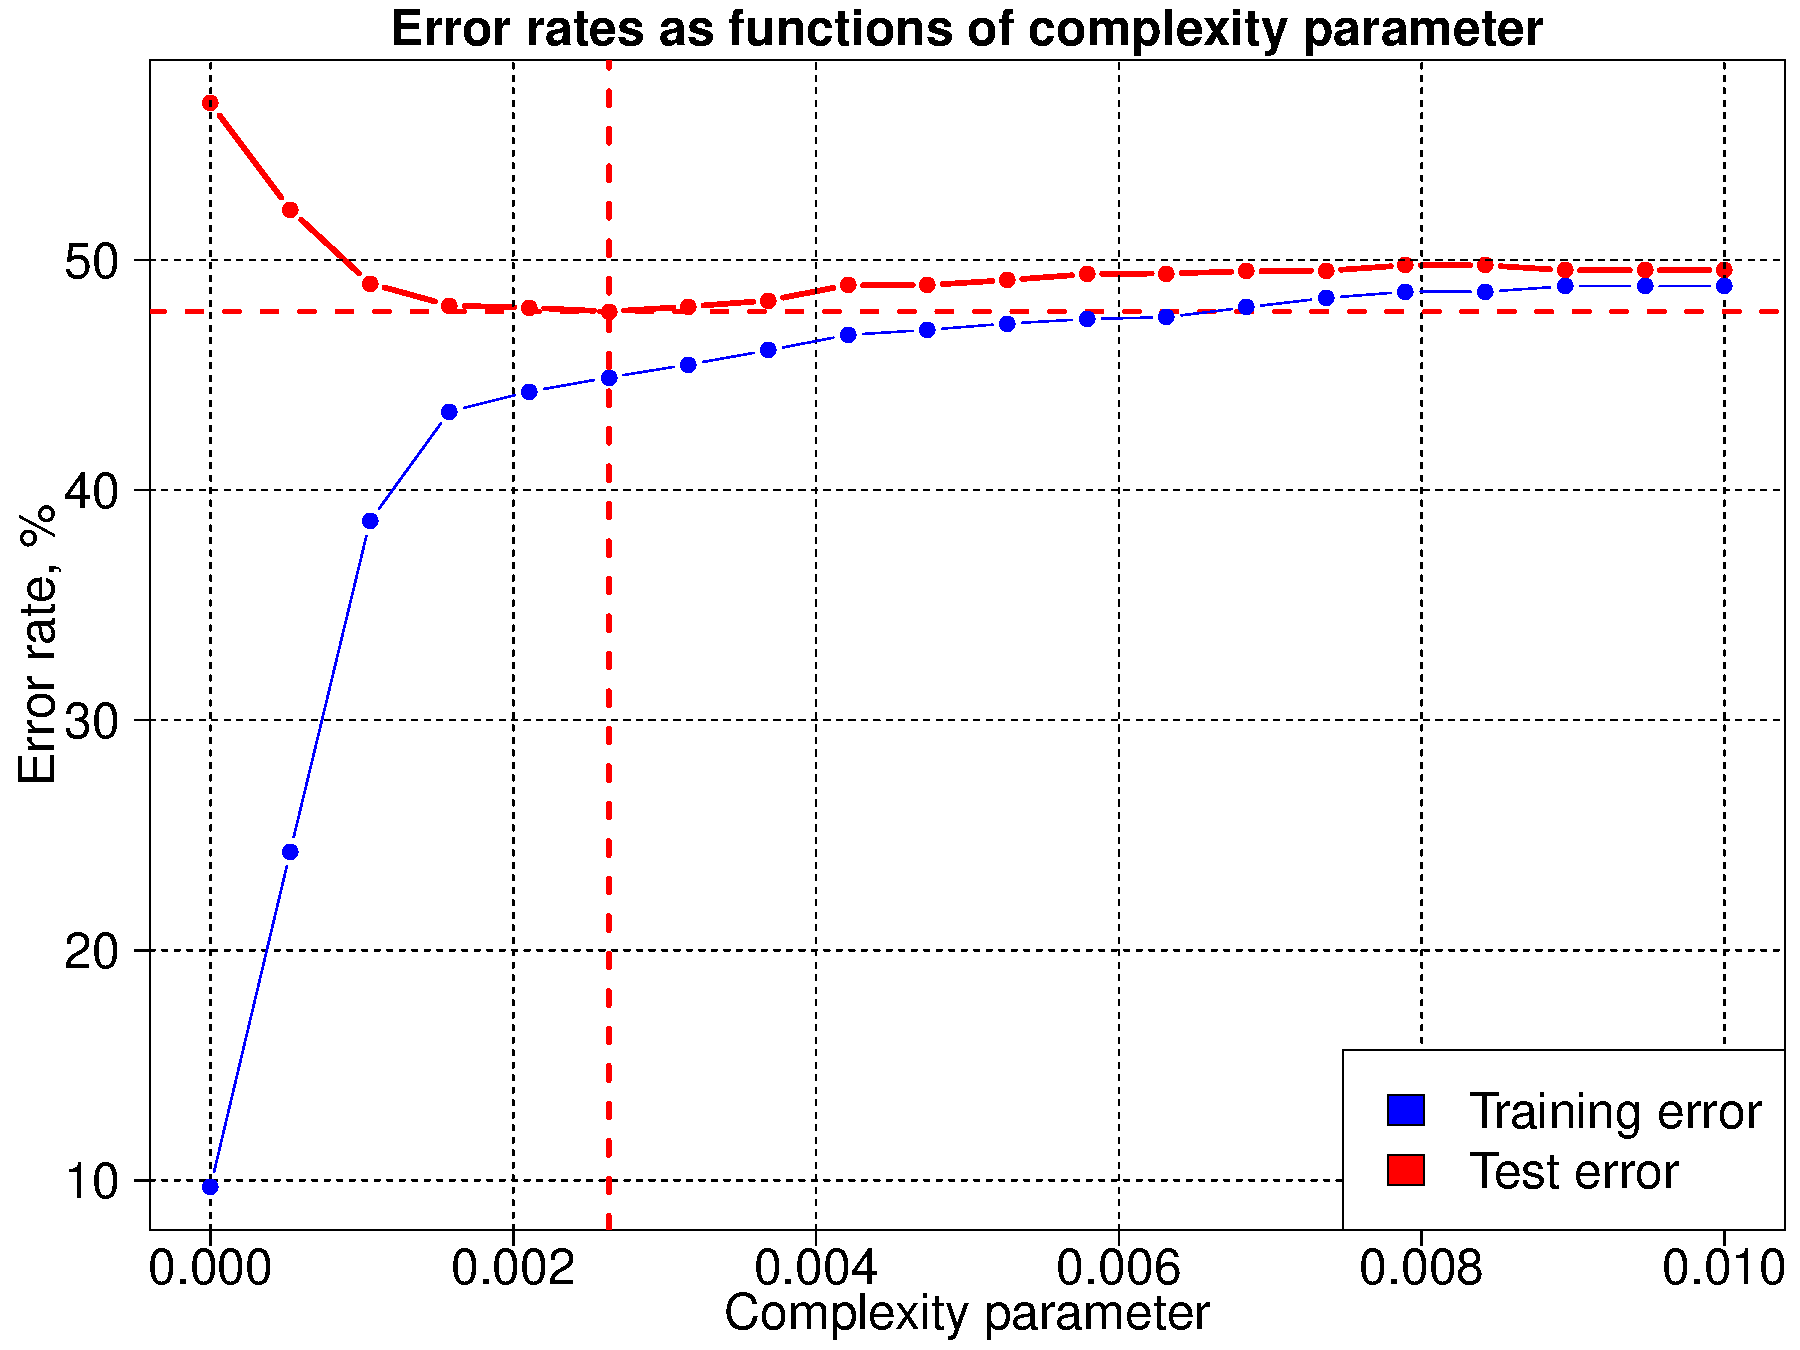
\includegraphics[width = 0.49\textwidth]{decision_tree_err_CV1.pdf}
  \caption{One layer 10-fold cross-validation applied to the
    dataset. Minimum number of observations in the node to attempt
    splitting was set to 5.  The optimal pruning level is 0.0026 and
    the error rate is 47.7 \%.}
  \label{fig:cv_1}
\end{figure}

Now this approach can be expanded to two layer cross-validation. In
the inner cross-validation loop the complexity parameter will be
selected and on the outer loop the performance of the best model will
be evaluated.  The procedure will produce information like this

\begin{figure}[htbp]
  \centering
  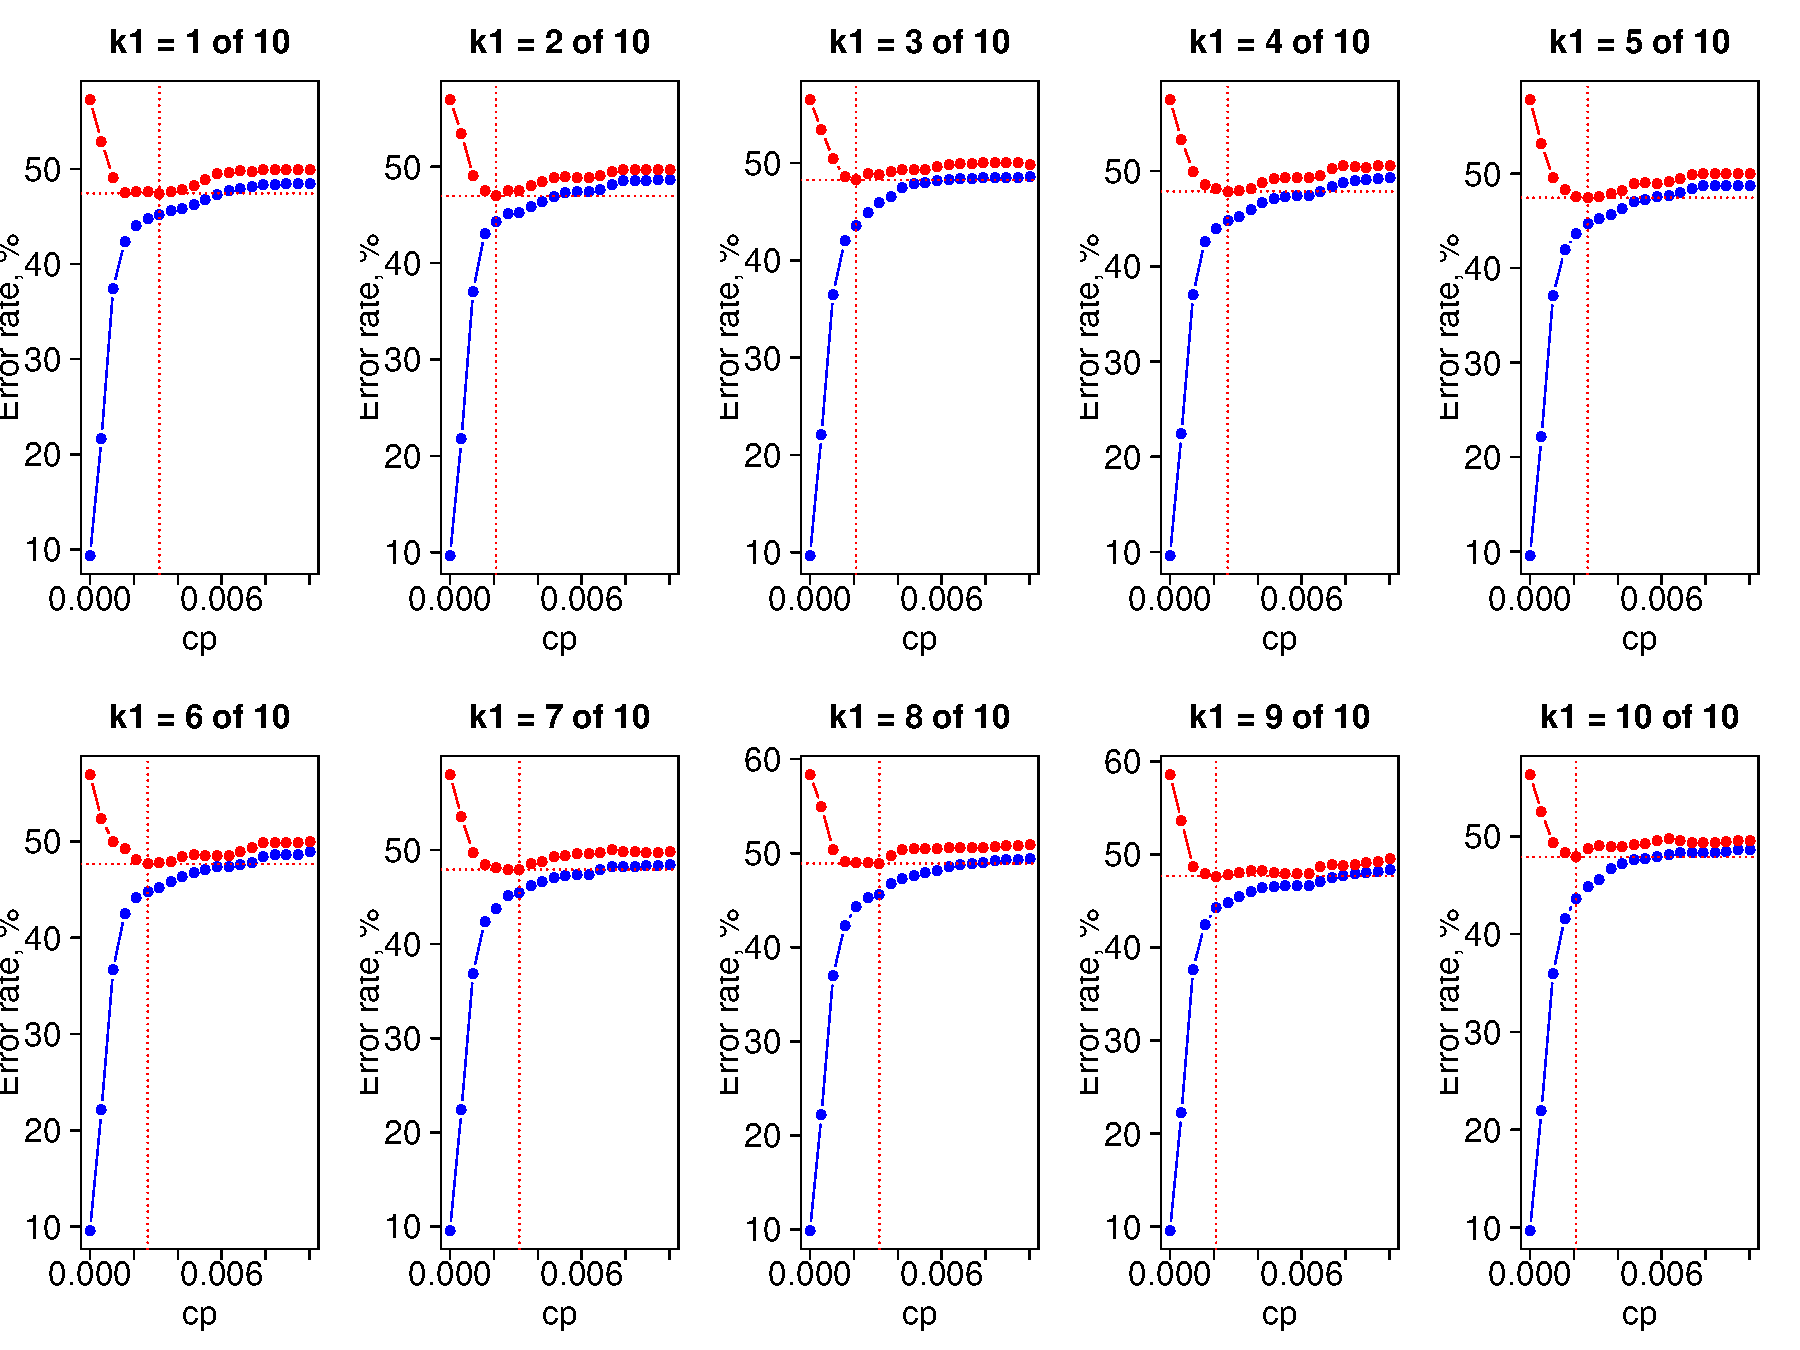
\includegraphics[width = 0.49\textwidth]{decision_tree_err_CV2.pdf}
  \caption{Two layer 10-by-10 cross-validation applied to the
    dataset. Minimum number of observations in the node to attempt
    splitting was set to 5.  The error rate is 47.8 \%.}
  \label{fig:cv_2}
\end{figure}

\subsection{K nearest neighbours}

Nearest neighbor classifier computes the distance to all data objects,
finds the nearest k data objects, and classifies according to the
majority of votes.  The basic application of the method is visualized
in Fig.~\ref{fig:knn_cv1}.  The optimal number of nearest neighbours
estimated by one layer 10-fold cross-validation is 23.

\begin{figure}[htbp]
  \centering
  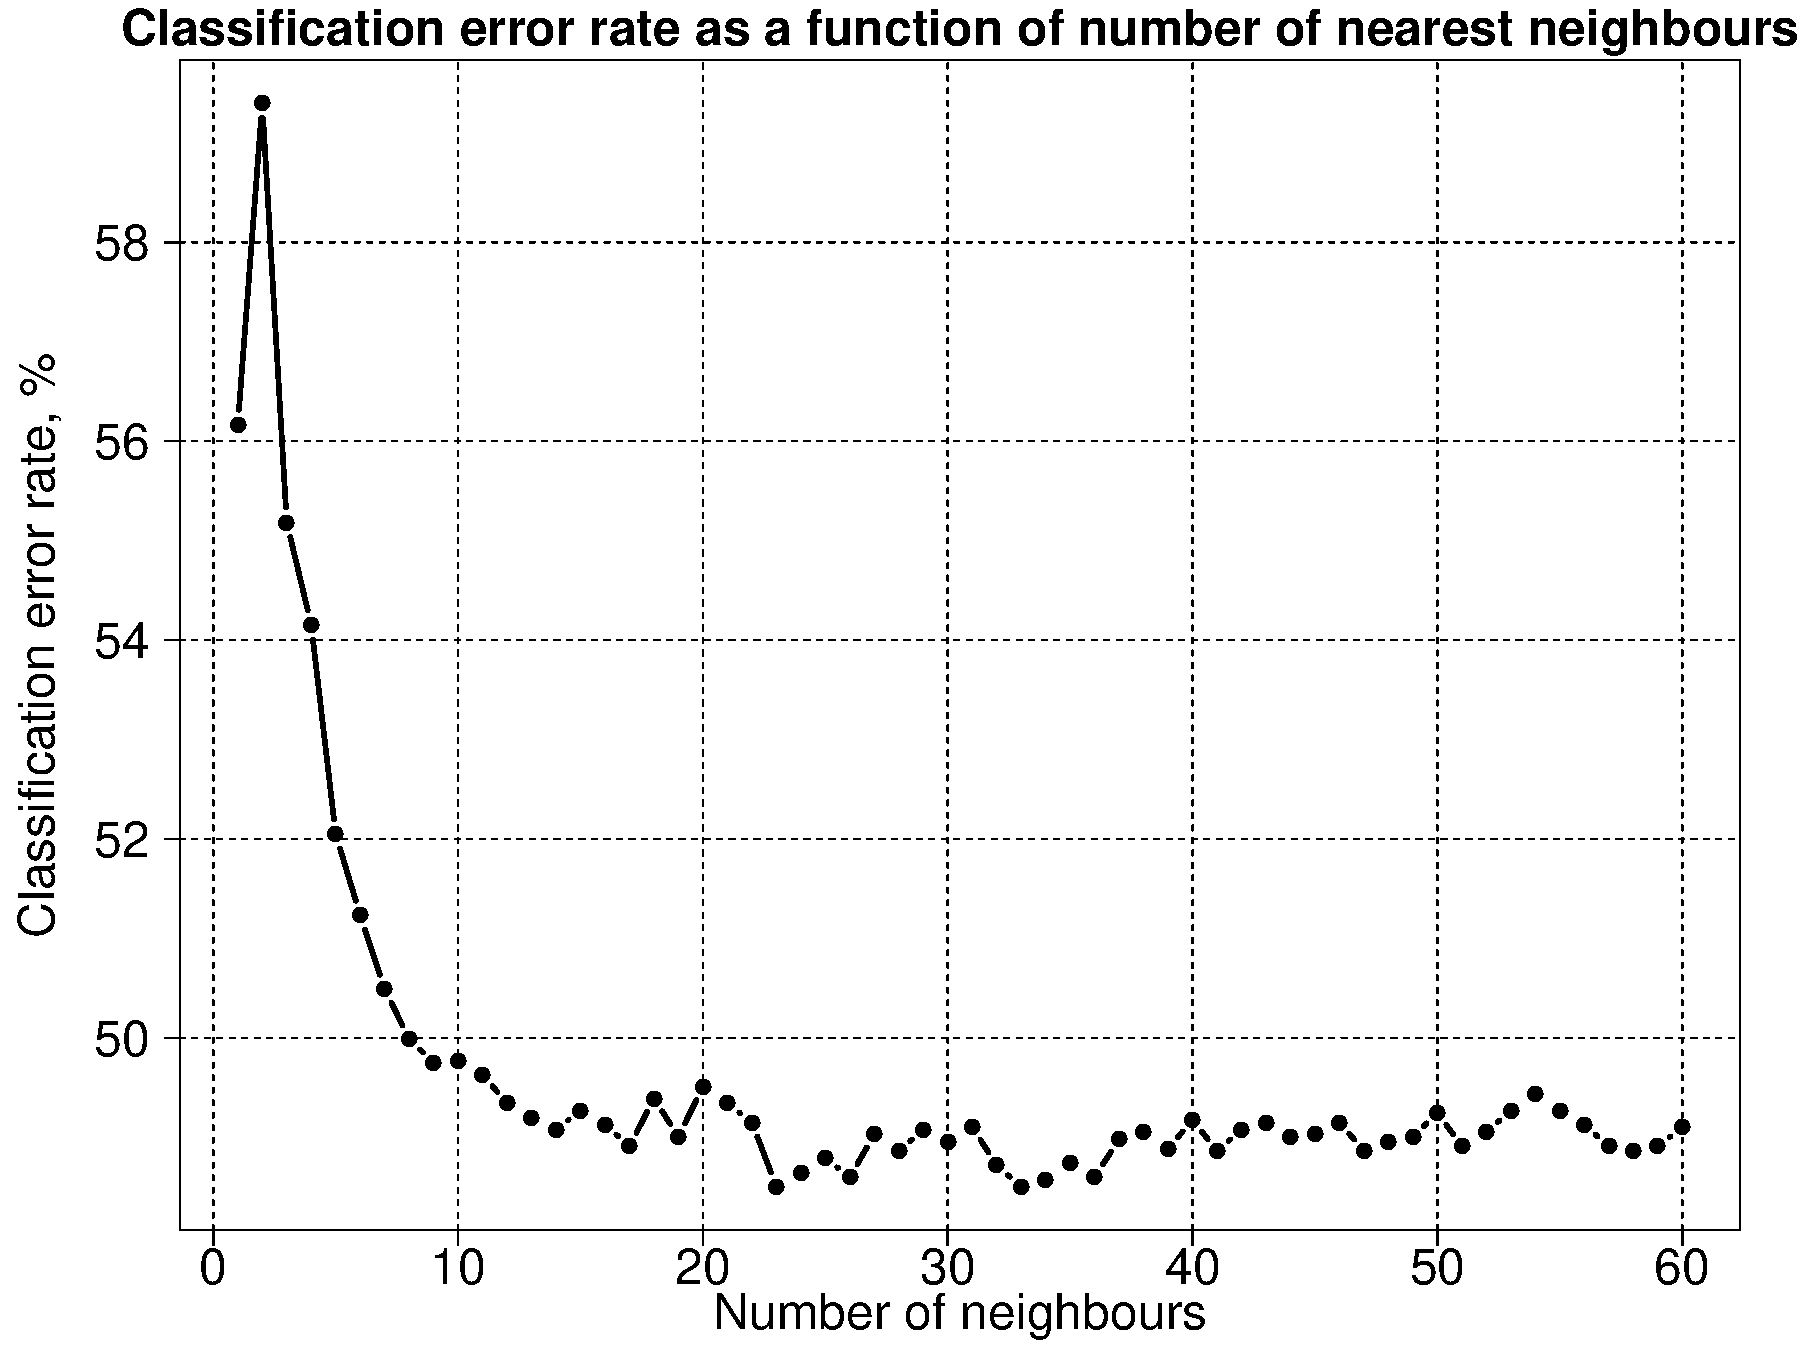
\includegraphics[width = 0.49\textwidth]{k_nearest_neighbours_err_CV1.pdf}
  \caption{One layer 10-fold cross-validation applied to the dataset.
    The optimal number of neighbours is 23 and the error rate is 50.01
    \%.}
  \label{fig:knn_cv_1}
\end{figure}

K nearest neighbor method applied in a two layer cross-validation loop
is presented in Fig.~\ref{fig:cv_2}.

\begin{figure}[htbp]
  \centering
  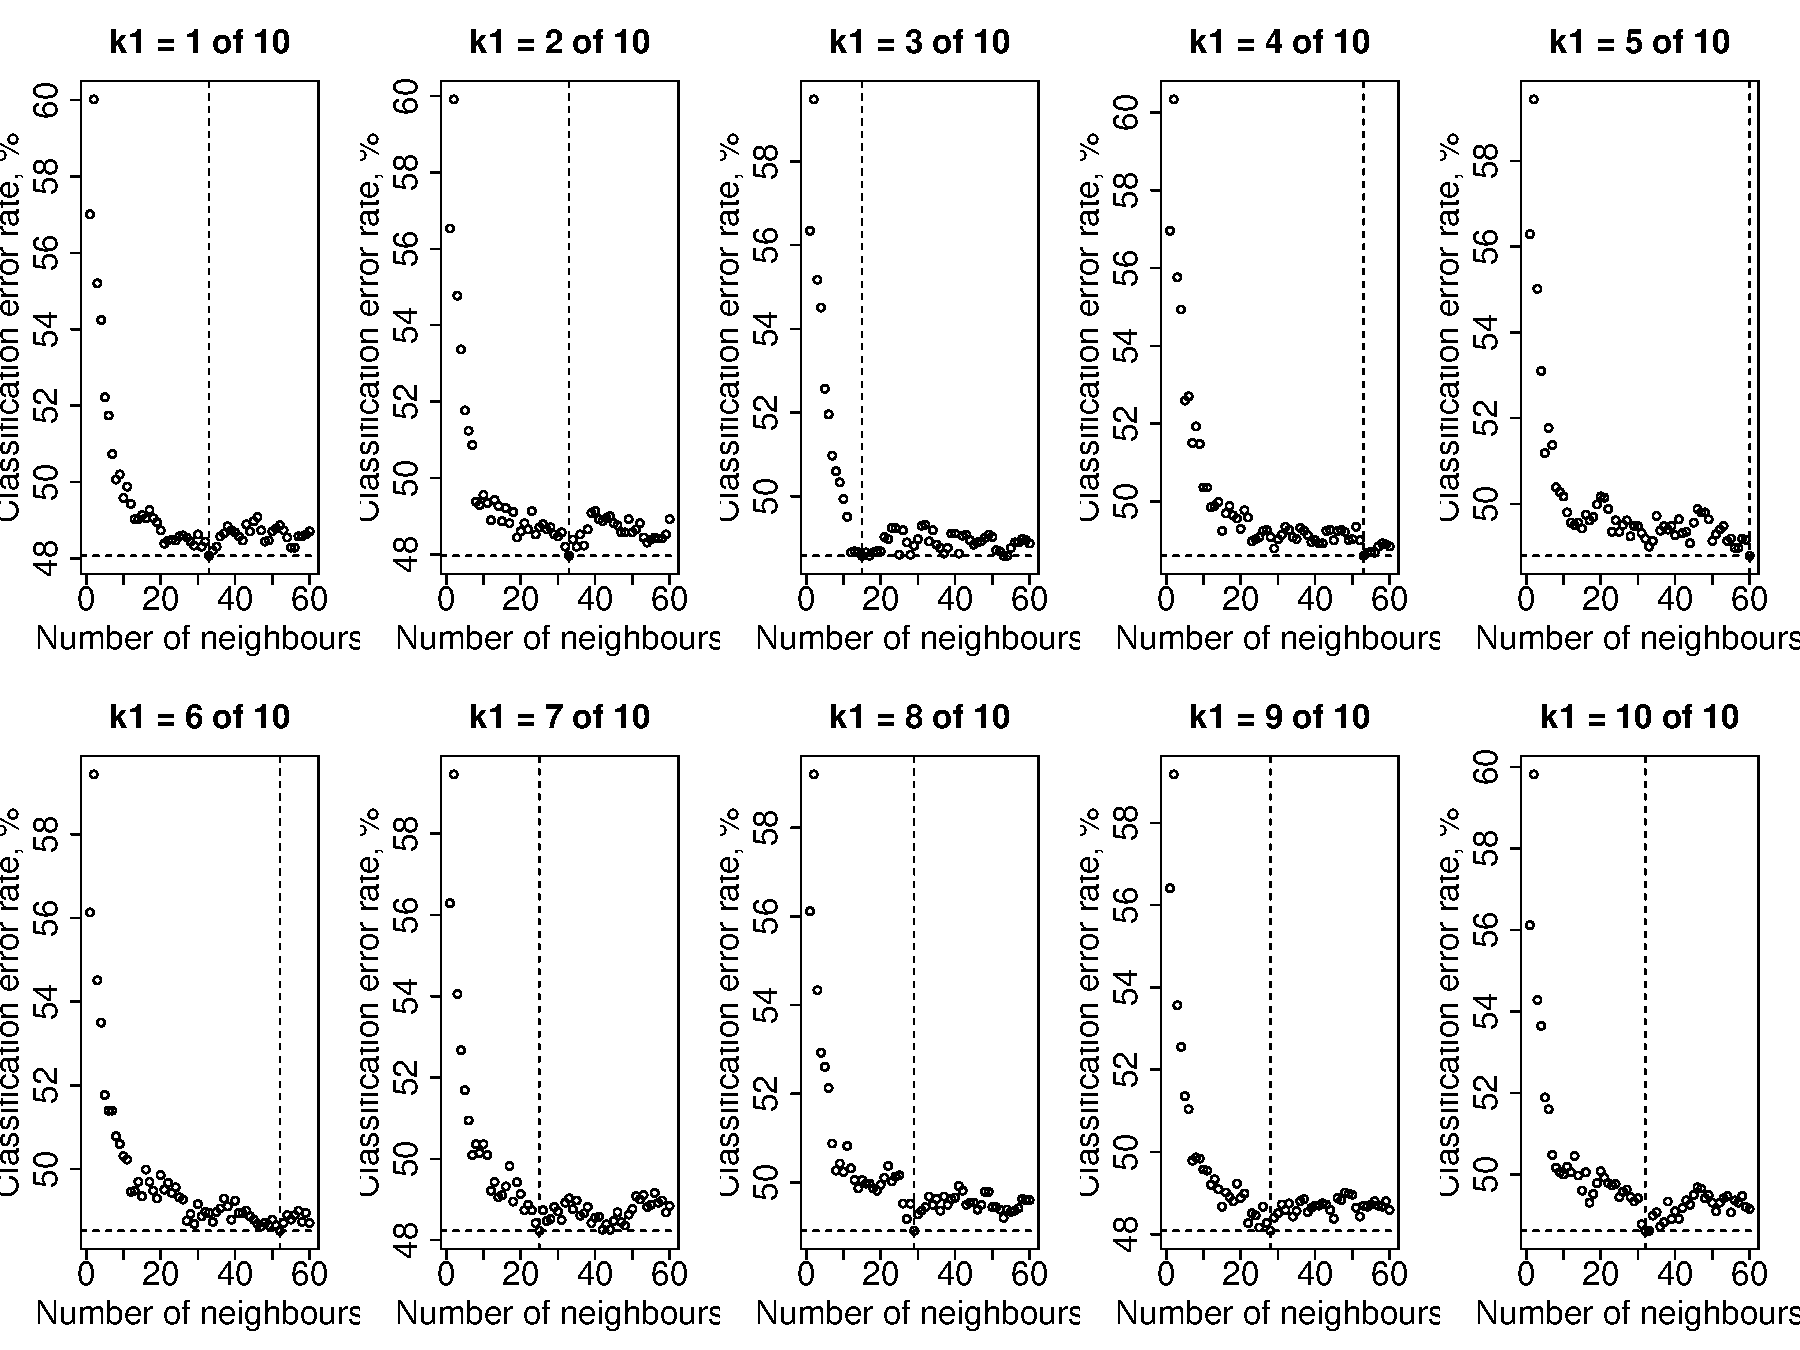
\includegraphics[width = 0.49\textwidth]{k_nearest_neighbours_err_CV2.pdf}
  \caption{Two layer 10-by-10 cross-validation applied to the
    dataset. The error rate is 49.25 \%}
  \label{fig:knn_cv_2}
\end{figure}


\subsection{Naive Bayes}

Naive bayes classifier gives the error rate of 54.41 \% with 10-fold
cross-validation.

There are two important aspects of classification and regression
methods, how well the methods can predict unlabeled data and how well
the method describe what aspects in the data causes the data to be
classified a certain way.


%%%%%%%%%%%%%%%%%%%% Results and Discussion %%%%%%%%%%%%%%%%%%%%
\section{Results and Discussion}
\label{sec:results_and_discussion}
If your data has previously been analyzed by regression or
classification in the lit- erature, please report what methods have
been used previously as well as their performance and relate your
results to these previous results.

Notice, if the analysis of your data is too computationally demanding
for choosing parameters in the inner cross-validation loop we suggest
you use the hold-out method instead of K-fold
cross-validation. Furthermore, if analyzing the data by ANN is too
computationally demanding you can consider only analyzing a subset of
your data by ANN.

The report should be 5-10 pages long including figures and tables and
give a precise and coherent account of the results of the regression
and classification methods applied to your data. Please hand in the
report by uploading it as a single, uncompressed .pdf file to
CampusNet no later than {\bf 12 April at 13:00}.  To ensure all group
members get credit for the report, put your names and study numbers on
the front page and ensure you upload the report as a group hand in and
put the name of your dataset on the front page.
%%%%%%%%%%%%%%%%%%%% Bibliography %%%%%%%%%%%%%%%%%%%%
\begin{thebibliography}{99}
\bibitem{Waugh.thesis} S.~Waugh,''Extending and Benchmark
  Cascade-Correlation,'' Thesis, 1997.
  \bibitem{Mayukh} H.~Mayukh, ``Age of Abalones using Physical
    Characteristics: A Classification Problem,'' ECE 539 Fall 2010
    Project Report, Department of Electrical and Computer Engineering
    University of Wisconsin-Madison, 2010.
\end{thebibliography}
\end{document}

%% \begin{lstlisting}[label = lst:logistic_regression, caption = {Results of logistic regression}]
%%   Call:
%% glm(formula = Class ~ Malaise + Ascites + Bilirubin + Histology, 
%%     family = binomial(link = logit), data = data)

%% Deviance Residuals: 
%%     Min       1Q   Median       3Q      Max  
%% -2.7029   0.2382   0.2888   0.4330   1.8019  

%% Coefficients:
%%             Estimate Std. Error z value Pr(>|z|)   
%% (Intercept)   1.2874     0.8407   1.531  0.12567   
%% Malaise       0.9020     0.5670   1.591  0.11162   
%% Ascites       1.9074     0.6621   2.881  0.00397 **
%% Bilirubin    -0.7838     0.2613  -3.000  0.00270 **
%% Histology    -0.9933     0.6132  -1.620  0.10529   
%% ---
%% Signif. codes:  0 ‘***’ 0.001 ‘**’ 0.01 ‘*’ 0.05 ‘.’ 0.1 ‘ ’ 1

%% (Dispersion parameter for binomial family taken to be 1)

%%     Null deviance: 145.117  on 144  degrees of freedom
%% Residual deviance:  91.903  on 140  degrees of freedom
%%   (10 observations deleted due to missingness)
%% AIC: 101.9

%% Number of Fisher Scoring iterations: 5
%% \end{lstlisting}
